% !TEX encoding = UTF-8
\documentclass[aspectratio=169,10pt]{beamer}

\usepackage[T2A]{fontenc}
\usepackage[utf8]{inputenc}
\usepackage[english,russian]{babel}
\usepackage{amsmath,amssymb}
\usepackage{graphicx}
\usepackage{booktabs}
\usepackage{array}
\usepackage{xcolor}
\usepackage{tikz}
\usetikzlibrary{arrows.meta,positioning,shapes.geometric}

\usetheme{Madrid}
\usecolortheme{beaver}

\setbeamertemplate{navigation symbols}{}
\setbeamertemplate{footline}{%
  \leavevmode%
  \hbox{%
  \begin{beamercolorbox}[wd=.5\paperwidth,ht=2.25ex,dp=1ex,center]{author in head/foot}%
    \usebeamerfont{author in head/foot}Т.\,Е.~Пономарев, БПМИ243%
  \end{beamercolorbox}%
  \begin{beamercolorbox}[wd=.5\paperwidth,ht=2.25ex,dp=1ex,center]{title in head/foot}%
    \usebeamerfont{title in head/foot}HS:BG RL \hspace{1em} \insertframenumber{} / \inserttotalframenumber%
  \end{beamercolorbox}}%
}

\setbeamerfont{frametitle}{size=\large,series=\bfseries}
\setbeamerfont{title}{size=\Large,series=\bfseries}
\setbeamercolor{frametitle}{fg=white,bg=red!60!black}
\setbeamercolor{title}{fg=red!60!black}
\setbeamercolor{structure}{fg=red!60!black}

\newcommand{\cit}[1]{\textcolor{gray!70!black}{\scriptsize[#1]}}

\title[RL в автобаттлерах]{Применение обучения с подкреплением\\в исследовании игр в автобаттлерах}
\author[Пономарев Т.\,Е.]{Пономарев Тимур Евгеньевич \\ \small БПМИ243}
\institute[НИУ ВШЭ]{%
  НИУ ВШЭ, Факультет компьютерных наук \\
  \small Руководители: к.ф.-м.н.\ П.\,В.~Кудеров, ст.~преп.\ М.\,К.~Горденко%
}
\date{Москва, 2026}

\begin{document}

% =================== 1. TITLE ===================
\begin{frame}
  \titlepage
\end{frame}

% =================== 2. TASK + MOTIVATION ===================
\begin{frame}{Мотивация}
  \textbf{Среда}: Hearthstone Battlegrounds (HS:BG) --- автобаттлер от Blizzard, {>}20\,млн игроков/мес.

  \vspace{0.3em}
  \begin{columns}[T]
    \column{0.52\textwidth}
    \textbf{Две фазы:}
    \begin{itemize}\small
      \item \textbf{Recruit}: покупка/продажа юнитов, reroll, апгрейд таверны, расстановка
      \item \textbf{Combat}: автоматический бой двух досок
    \end{itemize}

    \column{0.48\textwidth}
    \textbf{Почему интересно как RL-задача:}
    \begin{itemize}\small
      \item Богатый testbed: \textbf{POMDP + стохастика + комбинаторный action space + экономическое планирование}
      \item Структурно богаче Pokemon \cit{Guo, RLC 2025} --- есть экономика и позиционирование
      \item Жанр живой: Blizzard добавляет карты каждый сезон $\Rightarrow$ бенчмарк растёт вместе со средой
    \end{itemize}
  \end{columns}

  \vspace{0.5em}
  \textbf{Цель}: разработать исследовательскую платформу и обучить агента, способного вырабатывать конкурентоспособную стратегию в автобаттлерах.
\end{frame}

% =================== 3. MDP ===================
\begin{frame}{Формализация: POMDP}
  \[
    \mathcal{M} = (\mathcal{S}, \mathcal{A}, P, R, \gamma),\qquad \gamma = 0.99
  \]

  \begin{columns}[T]
    \column{0.55\textwidth}
    \textbf{$\mathcal{S} = \mathbb{R}^{1009}$} --- структурированное наблюдение:
    \vspace{0.2em}
    \small
    \begin{tabular}{lr}
      \toprule
      Компонент & Размер \\
      \midrule
      Global (HP, золото, тир, флаги) & 7 \\
      Board ($7 \times 37$) & 259 \\
      Hand ($10 \times 37$) & 370 \\
      Store ($7 \times 37$) & 259 \\
      Discover ($3 \times 37$) & 111 \\
      Enemy info & 3 \\
      \midrule
      \textbf{Итого} & \textbf{1\,009} \\
      \bottomrule
    \end{tabular}
    \normalsize

    \column{0.45\textwidth}
    \textbf{$\mathcal{A} = \text{Discrete}(32)$} с динамической маской:
    \vspace{0.2em}
    \begin{itemize}\small
      \item 0: End Turn
      \item 1: Roll
      \item 2--8: Buy / Target
      \item 9--15: Sell
      \item 16--25: Play Hand
      \item 26--31: Swap
    \end{itemize}

    \vspace{0.4em}
    \textbf{$R$}: terminal $\pm 5$, $r_{combat}$, $r_{synergy}$, $r_{board}$, $r_{economy}$
  \end{columns}
\end{frame}

% =================== 4. WHY HARD + GAP ===================
\begin{frame}{Почему задача нетривиальна + gap в литературе}
  \begin{columns}[T]
    \column{0.5\textwidth}
    \textbf{Что делает задачу сложной:}
    \begin{itemize}
      \item \textbf{POMDP}: доска оппонента видна только в бою
      \item \textbf{Стохастика}: атаки рандомны, reroll рандомен
      \item \textbf{Комбинаторика}: $C_{18}^{7} \cdot 7! \sim 1.6\cdot 10^{8}$ конфигураций доски
      \item \textbf{Sparse reward}: итог через 10--15 раундов (credit assignment)
      \item Конечный пул карт, конкуренция игроков
    \end{itemize}

    \column{0.5\textwidth}
    \textbf{Существующие open-source среды:}
    \begin{itemize}
      \item \textbf{Fireplace} --- классический HS, нет BG
      \item \textbf{Unity ML-Agents} --- 10--50 игр/с (графика)
      \item \textbf{HSReplay / Firestone} --- только реплеи, нет интеракции
      \item \textbf{Leiden} \cit{Ren 2022}, \textbf{LUT} \cit{Zhang 2024} --- упрощения: без аур, Discovery, позиций
    \end{itemize}

    \vspace{0.5em}
    $\Rightarrow$ \textbf{пишем собственный движок с полной боевой системой}
  \end{columns}
\end{frame}

% =================== 5. SIMULATOR (MINE) ===================
\begin{frame}{Симулятор HS:BG \hfill {\small\normalfont реализовано мной}}
  \textbf{$\sim$3\,500 LOC движка + 839 LOC Gymnasium-обёртки}, 11 модулей, 13 тестовых модулей (цифры из отчёта). Существующие open-source BG-среды (Leiden 2022, LUT 2024) используют упрощённые правила --- без аур, Discovery, цепных Deathrattle, позиционных эффектов. \textbf{Моя --- наиболее полная по охвату механик} на момент написания отчёта.

  \vspace{0.3em}
  \begin{columns}[T]
    \column{0.52\textwidth}
    \textbf{Подсистемы:}
    \begin{itemize}\small
      \item \textbf{Entities}: Buff Layer Stack (5 слоёв)
      \item \textbf{Event System}: приоритизированная очередь, 17 типов событий, детерминированная сортировка $(\text{group},\,\text{priority},\,\text{side},\,\text{slot},\,\text{uid})$
      \item \textbf{Combat}: 10 механик (Deathrattle, Reborn, Divine Shield, Cleave, Poisonous, Windfury, Taunt, Magnetize, Avenge, Immediate Attack)
      \item \textbf{Auras}: stateless пересчёт
      \item \textbf{Tavern}: Buy/Sell, Triples, Discovery, Spells, Freeze, Tier-up
      \item \textbf{Gym wrapper}: Action Masking, детерминизм
    \end{itemize}

    \column{0.48\textwidth}
    \footnotesize
    \textbf{Buff Layer Stack:}
    \begin{tabular}{p{2.5cm}p{3.5cm}}
      \toprule
      \textbf{Слой} & \textbf{Время жизни} \\
      \midrule
      Базовый & неизменяемый \\
      Перманентный & навсегда \\
      Ходовой & до конца хода \\
      Боевой & до конца боя \\
      Аурный & пересчёт при любом изменении доски \\
      \bottomrule
    \end{tabular}
    \normalsize

    \vspace{0.5em}
    \small Аналогов в open-source не обнаружено.
  \end{columns}
\end{frame}

% =================== 6. ARCH: MLP vs TRANSFORMER ===================
\begin{frame}{Архитектуры: MLP vs Transformer --- обоснование}
  \textbf{MLP на плоском $\mathbb{R}^{1009}$}: не видит границы зон, не ловит set-взаимодействия (синергии, Baron+Deathrattle), тратит параметры на padding.

  \vspace{0.3em}
  \textbf{Токенизация $\mathbb{R}^{1009}$ для Transformer:}
  \small
  \begin{itemize}\itemsep0pt
    \item \textbf{27 entity-токенов}: Board\,(7) + Hand\,(10) + Store\,(7) + Discover\,(3), каждый слот $\to$ 37 признаков
    \item \textbf{+\,1 [GLOBAL\_CTX] токен}: $\text{MLP}(\text{Global}_7 \oplus \text{Enemy}_3) \in \mathbb{R}^{d_{\text{model}}}$
    \item $\Rightarrow$ \textbf{28 токенов $\times$ 128} $\to$ DecomposedEncoder $\to$ FiLM $\to$ 4 $\times$ GTrXL $\to$ PMA $\to$ features
  \end{itemize}
  \normalsize

  \vspace{0.2em}
  \textbf{Компоненты} (все из state-of-the-art 2018--2024):
  \footnotesize
  \begin{tabular}{p{3.6cm}p{10.2cm}}
    \toprule
    DecomposedEncoder \cit{MARL-GPT 2024} & раздельные проекции continuous / binary / race $\to$ суммирование \\
    FiLM $(\gamma+1)\odot x + \beta$ \cit{Perez 2018} & мультипликативная модуляция токенов глобальным контекстом \\
    {[GLOBAL\_CTX]} \cit{AlphaStar 2019} & карты \emph{обращаются} к макро-контексту внутри Attention \\
    GTrXL-шлюз \cit{Parisotto 2020} & $b_{\text{init}}{=}{-}3$: шлюз закрыт на старте, градиенты открывают постепенно \\
    Multi-Seed PMA \cit{Set Transformer 2019} & $K{=}4$ seed-векторов: агрегация множества карт переменного размера \\
    \bottomrule
  \end{tabular}
  \normalsize

  \vspace{0.2em}
  $\sim$600\,k параметров. \textbf{Компоненты известны из литературы, но собраны вместе под автобаттлеры впервые.}
\end{frame}

% =================== 7. RESULT 1: SAMPLE EFFICIENCY ===================
\begin{frame}{Результат 1: Sample Efficiency \hfill {\small\normalfont главный}}
  \begin{columns}[T]
    \column{0.5\textwidth}
    \centering
    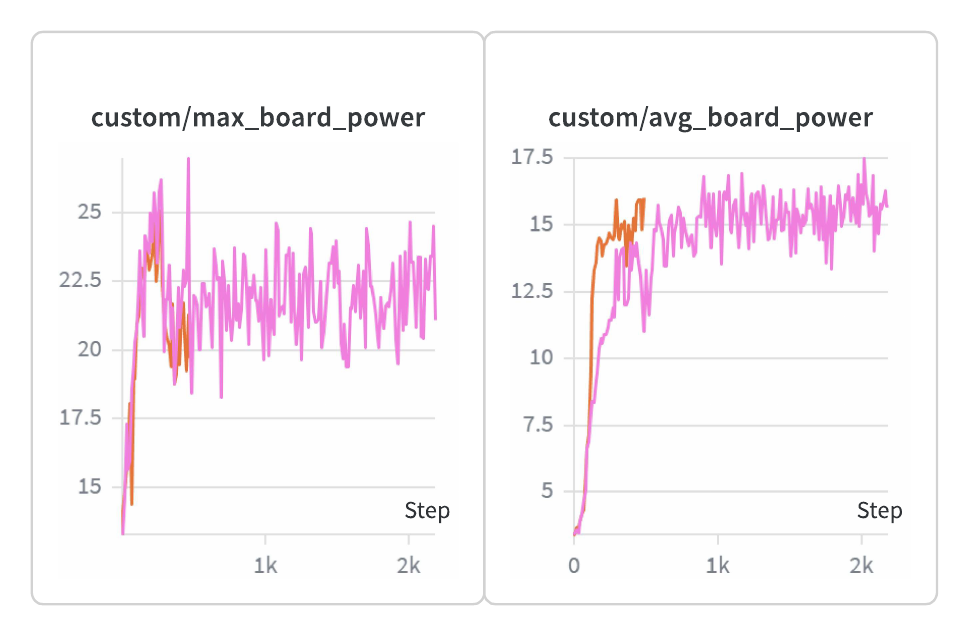
\includegraphics[width=\textwidth]{wandb-p4.png}
    \\ \scriptsize\textit{WandB: custom/max\_board\_power и custom/avg\_board\_power.\\Transformer --- оранжевая (обучение остановлено на 300k шагов), MLP --- розовая (1.5M шагов)}

    \column{0.5\textwidth}
    \footnotesize
    \begin{tabular}{p{3.3cm}rr}
      \toprule
      & \textbf{MLP} & \textbf{Transformer} \\
      \midrule
      Шаги до плато & 400k & \textbf{80k} \\
      Inference FPS & 1200 & 250 \\
      Wall-clock & 333 с & 320 с \\
      \bottomrule
    \end{tabular}

    \vspace{0.3em}
    \textbf{Ускорение $\sim\mathbf{5\times}$ по sample efficiency.}

    \vspace{0.5em}
    \textbf{Три фазы обучения} (Transformer в $\sim$5\,раз быстрее):
    \begin{enumerate}
      \item тратить золото
      \item синергии и триплеты
      \item финальная шлифовка
    \end{enumerate}

    \vspace{0.3em}
    \textbf{Про FPS}: MLP compute-bound на мелких матрицах (GPU простаивает), Transformer честно грузит GPU и масштабируется. \textbf{С ростом compute Transformer будет только быстрее MLP.}
    \normalsize
  \end{columns}
\end{frame}

% =================== 8. RESULT 2: PvP ===================
\begin{frame}{Результат 2: PvP --- Transformer vs MLP}
  \textbf{Прямое столкновение обученных агентов} (MLP 1.5M шагов, Transformer 300k):

  \vspace{0.3em}
  \centering
  \begin{tabular}{cccc}
    \toprule
    \textbf{Игра} & \textbf{HP Transformer} & \textbf{HP MLP} & \textbf{Результат} \\
    \midrule
    1 & 22 & 21 & таймаут \\
    2 & 30 & 25 & таймаут \\
    3 & 24 & 27 & таймаут \\
    \bottomrule
  \end{tabular}

  \vspace{0.5em}
  \raggedright
  \textbf{Все три партии ушли в таймаут} ($>$\,500 ходов). Ни один агент не смог добить другого.

  \vspace{0.3em}
  \textbf{Интерпретация:}
  \begin{itemize}\small
    \item Обе архитектуры \textbf{``решили'' текущую среду}: при 18 картах и тирах 1--3 пространство стратегий слишком узкое
    \item Движок работает корректно: нет эксплойтов, стабильное равновесие
    \item \textbf{Мотивация для продолжения}: расширить пул карт и тиры (см. апдейты)
  \end{itemize}
\end{frame}

% =================== 9. RESULT 3: ATTENTION ===================
\begin{frame}{Валидация Transformer: attention по слоям}
  \begin{columns}[T]
    \column{0.78\textwidth}
    \centering
    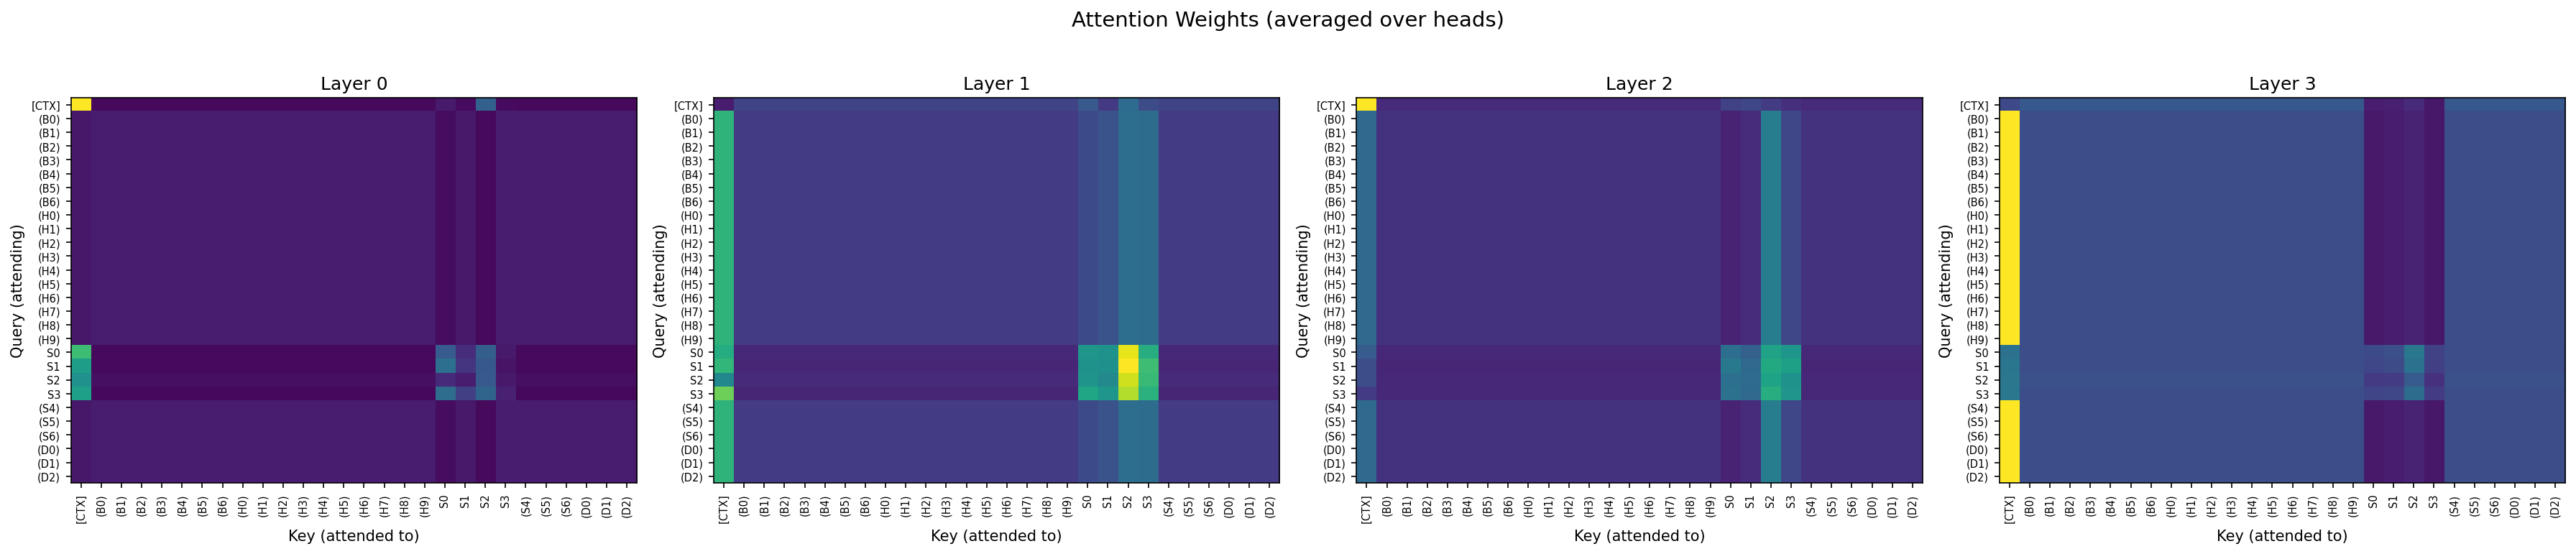
\includegraphics[width=\textwidth]{attention_avg_by_layer.png}

    \column{0.22\textwidth}
    \scriptsize
    \textbf{Что видно:}
    \begin{itemize}
      \item \textbf{Layer 0}: доска смотрит сама на себя + на [CTX]
      \item \textbf{Layer 3}: доска $\leftrightarrow$ магазин (cross-zone)
    \end{itemize}

    \vspace{0.4em}
    \textbf{Вывод}: сеть учит \emph{осмысленные} взаимодействия, а не шум.
    \normalsize
  \end{columns}
\end{frame}

% =================== 9b. RESULT 3: ATTENTION HEADS ===================
\begin{frame}{Валидация Transformer: специализация голов Layer 0}
  \begin{columns}[T]
    \column{0.78\textwidth}
    \centering
    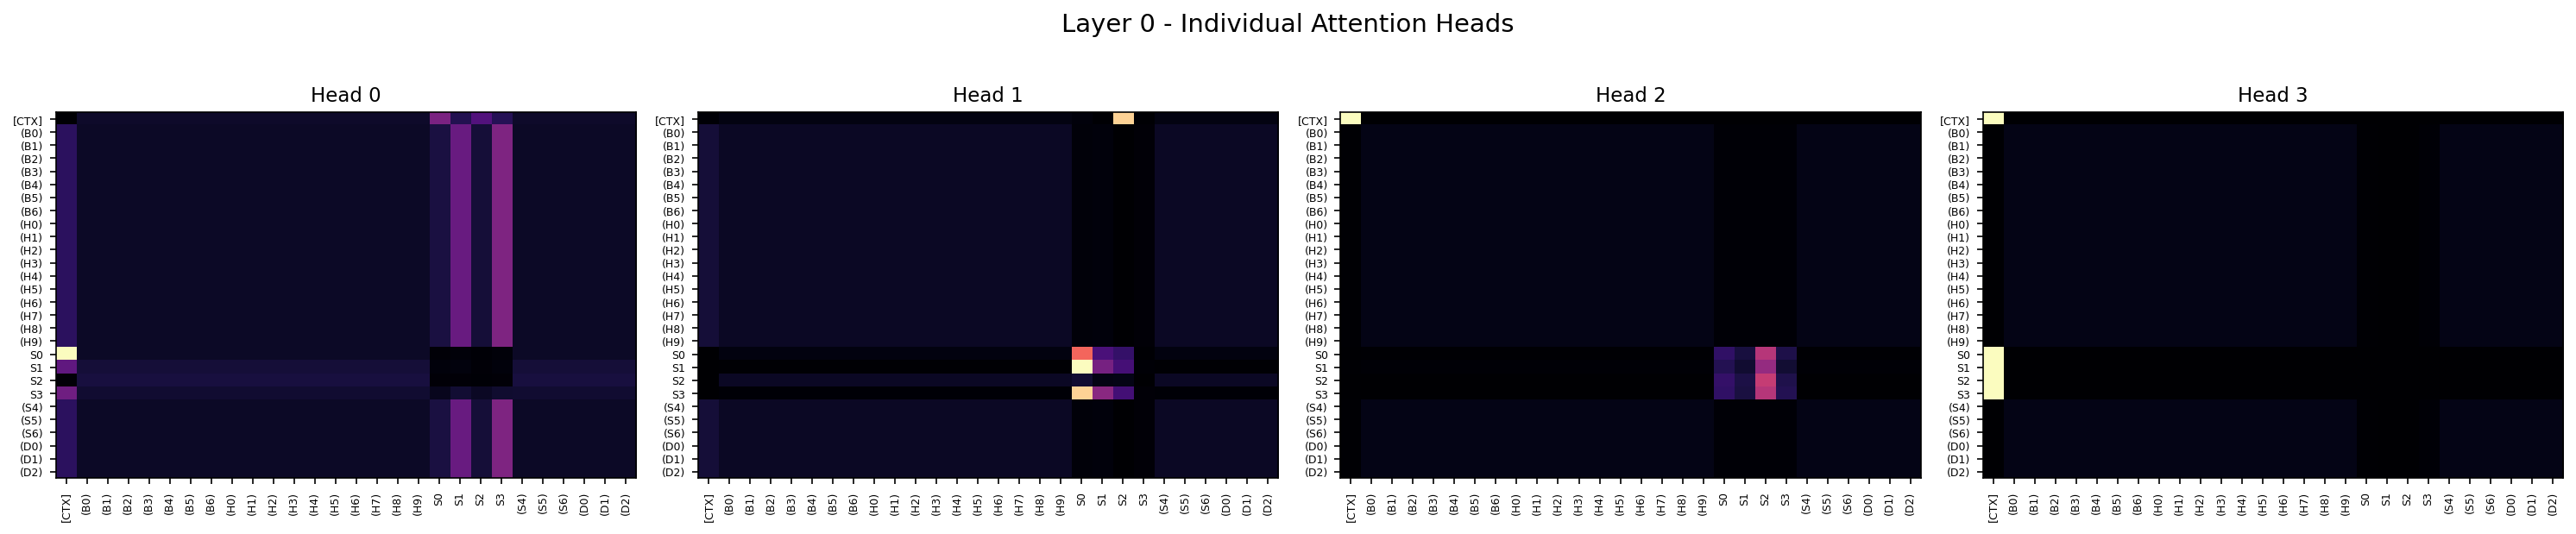
\includegraphics[width=\textwidth]{attention_heads_layer0.png}

    \column{0.22\textwidth}
    \scriptsize
    \textbf{Головы \emph{специализировались}:}
    \begin{itemize}
      \item Head 0: внутри доски
      \item Head 1: магазин
      \item Head 3: [CTX] + Discovery
    \end{itemize}

    \vspace{0.4em}
    Никто не заставлял --- PPO gradient нашёл разделение труда сам.
    \normalsize
  \end{columns}
\end{frame}

% =================== 10. REWARD + ABLATION HONESTY ===================
\begin{frame}{Reward design --- эмпирический путь}
  Reward shaping в sparse-средах --- \textbf{признанная открытая задача RL} \cit{Sutton \& Barto; Ng 1999 PBRS; Andrychowicz HER 2017}.

  \vspace{0.3em}
  \textbf{Что пробовали:}
  \begin{enumerate}\small
    \item \textbf{5-компонентный shaping} (в отчёте): $r = r_{combat} + r_{economy} + r_{board} + r_{terminal} + r_{synergy}$ --- работал на малом пуле карт
    \item \textbf{MC Oracle PBRS} --- dense reward через C++ Monte-Carlo симуляцию исходов боёв. Ради него написан C++-порт combat (7\,412 боёв/с). При росте пула значимого выигрыша не дал
    \item \textbf{Sparse + tier-based curriculum} --- текущий подход: агент начинает с тиров 1--2, пул расширяется по мере сходимости
  \end{enumerate}

  \vspace{0.3em}
  \textbf{Частичный ablation:} MLP vs Transformer + три конфигурации reward. \textbf{В рамках вычислительного бюджета данного исследования полная покомпонентная абляция нецелесообразна}; фокус сделан на proof-of-concept архитектуры и валидации sample efficiency. Выбор компонент обоснован литературным обзором 60+ работ (см.\ \texttt{theory/transformer\_scaling\_research.md}).
\end{frame}

% =================== 11. AFTER REPORT + FUTURE ===================
\begin{frame}{Работа продолжается: апдейты после отчёта + Future Work}
  \begin{columns}[T]
    \column{0.5\textwidth}
    \textbf{Сделано после сдачи отчёта:}
    \begin{itemize}\small
      \item Пул карт расширен с $\sim$18 до \textbf{175 карт, тиры 1--7}
      \item Combat engine портирован на \textbf{C++ через pybind11}: 7\,412 боёв/с (изначально ради MC Oracle)
      \item \textbf{Tier-based curriculum learning}: \texttt{HearthstoneEnv(max\_tier)}
      \item \textbf{Categorical Critic} (DreamerV3): 255 бинов, symlog two-hot, cross-entropy loss
      \item \textbf{Кодовая база выросла}: с 3.5\,k LOC до $\sim$10.7\,k Python + 3.7\,k C++ + 9.8\,k тестов; тестов --- с 13 до \textbf{24 модулей / 762 теста}
    \end{itemize}

    \column{0.5\textwidth}
    \textbf{Future Work:}
    \begin{itemize}\small
      \item \textbf{Авторегрессионный action space} SAINT \cit{Wen 2025} + Pointer Networks \cit{Vinyals 2015}
      \item \textbf{RMCTS} \cit{Luo 2025} + Latent Battle Predictor (MuZero-style \cit{Schrittwieser 2020})
      \item Пайплайн \textbf{BC $\to$ PPO $\to$ Self-Play} по образцу Pokemon \cit{Guo RLC 2025}
      \item \textbf{Opponent modeling}: байесовский классификатор архетипов, DTQN \cit{Esslinger 2022} для памяти
    \end{itemize}
  \end{columns}
\end{frame}

% =================== 12. CONCLUSIONS ===================
\begin{frame}{Результаты, выносимые на защиту}
  \begin{enumerate}
    \item \textbf{Headless-среда HS:BG с наиболее полным охватом механик}: 10 боевых механик (Deathrattle, Reborn, Divine Shield, Cleave, Poisonous, Windfury, Taunt, Magnetize, Avenge, Immediate Attack), приоритизированная event-система, ауры, экономика, Action Masking, Gymnasium-API. \textbf{$\sim$3\,500 LOC движка + 839 LOC env} (по отчёту). В отличие от существующих работ (Leiden 2022, LUT 2024), реализованы ауры, Discovery и позиционные эффекты.

    \vspace{0.3em}
    \item \textbf{Transformer-экстрактор под автобаттлеры}: DecomposedEncoder + FiLM + [GLOBAL\_CTX] + GTrXL + Multi-Seed PMA. Компоненты взяты из state-of-the-art работ 2018--2025\,гг.\ (AlphaStar, Set Transformer, GTrXL, MARL-GPT). Для жанра автобаттлеров attention-based экстрактор с таким охватом компонент --- новая сборка.

    \vspace{0.3em}
    \item \textbf{Экспериментальная валидация на реальных WandB-логах}: Transformer достигает того же плато в \textbf{$\sim 5\times$ быстрее} по sample efficiency (80k vs 400k шагов). Attention-анализ показал \emph{самоорганизованную специализацию голов}: head~0 --- внутри доски, head~1 --- магазин, head~3 --- глобальный контекст.
  \end{enumerate}

  \vspace{0.6em}
  \centering
  \large\textbf{Спасибо за внимание}
\end{frame}

\end{document}
